\documentclass[10pt]{article}
\usepackage{graphicx}
\usepackage{amssymb}
\usepackage{amsmath}
\usepackage{lipsum}
\usepackage{biblatex}

\usepackage{post}

\addbibresource{bibfile.bib}
\title{A Review of Karmakar's Algorithm}
\author{}
\date{}



\begin{document}
\onecolumn
\maketitle
\begin{quote}
N. Karmakar's 1984 paper \citetitle{karmarkar1984new} gave a very efficient polynomial time  interior programming algorithm for solving  linear optimization problem. The algorithm given by  Khachiyan \cite{khachiyan1980polynomial} although  proved existence polynomial time algorithms for linear programming, but these were very in efficient in practice. The simplex algorithm, although proved to be of worst case exponential complexity \cite{goldfarb1994complexity}, was doing well in practice.
\end{quote}

\begin{center}This post is a review of Narendra Karmarkar's original paper \cite{karmarkar1984new}.
\end{center}
\noindent{}The paper starts out to solve a Linear programing problem restricted with several assumptions which are enumerated below. 
\begin{description}
\item[Assumption 1] The problem to be solved is of following format
\begin{align}
&\text{minimise} &&c^Tx\;,\; c,x\in \mathbb{R}^n \label{eqn:restrictivelp}\\
&\text{subjected to} &&x\in \Omega\cap S\;\text{where}\nonumber\\
&&&\Omega =\{x|Ax=0\}\nonumber\\
&&&S = \{x|x\geq0,\sum x_i = 1\}\nonumber
\end{align}
\item[Assumption 2] Minimum value of the objective function $c^Tx$ is $0$
\item[Assumption 3] The problem is feasible and center of simplex $S$, given by $a_o = \vec{1}/n$ is a feasible starting point.
\end{description}

These assumptions are eventually removed by providing easy methods to cast any LP problem into the restrictive form specified in Eq.~\ref{eqn:restrictivelp}

\section{A different problem and its easy solution}
Consider the following problem
\begin{align*}
&\text{minimise} &&c^Tx\;,\; c,x\in \mathbb{R}^n\\
&\text{subjected to} &&x\in \Omega\cap E\;\text{where}\\
&&&\Omega =\{x|Ax=b\}\\
&&&E \text{ is an ellipsoid in $n$ dimensions}
\end{align*}
Note: $\Omega$ is an affine space.
%\begin{figure}[htbp]
%	\begin{center}
%	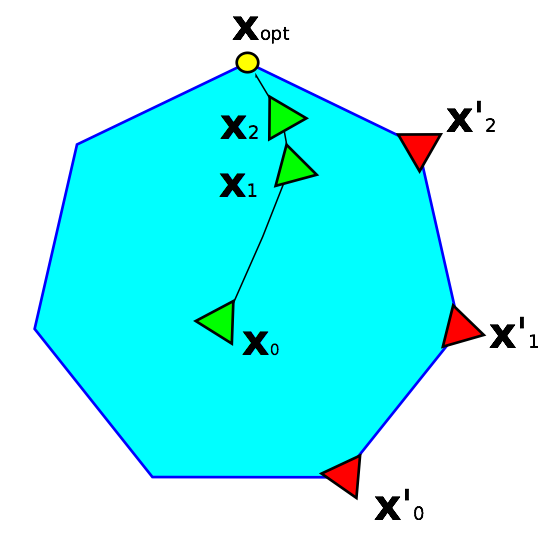
\includegraphics[width=5cm]{img.png}
%	\end{center}
%	\caption{A LP constrained by affine space and an Ellipsoid}
%\end{figure}


The solution of this problem is simple with the following idea. Apply a linear transformation $T$ to the entire problem space so that the ellipsoid becomes a sphere $S$. We have,
\begin{align*}
	E\mapsto S\hspace{1cm}
	\Omega \mapsto \bar{\Omega}\hspace{1cm}
	c \mapsto \bar{c}
\end{align*}
Affine spaces subjected to a linear transformation are still affine. So $\bar{\Omega}$ is still an affine space. Also intersection of an affine space and a sphere is a lower dimensional sphere. See Fig.~\ref{fig:sphereintersectionaffine}
\begin{figure}[htbp]
	\begin{center}
	\vspace{1cm}
	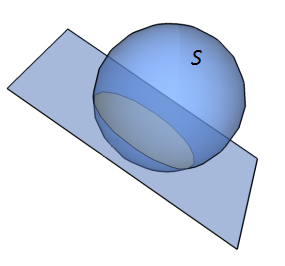
\includegraphics[width=8cm]{sphereintersectionaffine.png}
	\end{center}
	\caption{Intersection of Sphere and an Affine space is another sphere in lower dimension.}
	\label{fig:sphereintersectionaffine}
\end{figure}

Thus the above problem becomes 
\begin{align*}
&\text{minimise} &&\underline{c}^Tx\\
&\text{subjected to} &&x\in \underline{S}=S\cap \bar{\Omega}\;\text{, a sphere}
\end{align*}
$\underline{c}$ is $\bar{c}$ projected on to $\underline{S}$.


The solution of optimizing a linear function $\underline{c}^Tx$, constrained by a sphere is simple. From the center of the sphere, take a step of length equal to its radius in the direction $\underline{c}$.
\section{Back to the original problem}
Karmakar's algorithm works as follows.

Define a simplex $S=\{x| \sum x_i = 1 and x_i\geq 0, i=1,2,\dots,n+1\}$
Choose a point in the interior of the polytope Let this point be $a$.
\begin{description}
\item[Step 1] Define a projective transformation of the positive orthant $P^+$ (positive axis) space to $S$ such that image of point $a$ falls on center $a_0$ of the simplex.
\item[Step 2] Find the largest sphere that can be inscribed in $S$ with $a_0$ as its center. Let it be $B(a_o,r)$
\item[Step 3] Optimize the projection of the objective function, constrained by $B(a_0,r)$. 
Linear functions stays linear under projective transformations.
\item[Step 4]  Project the new point back to original space.
\end{description}

The projective transformation in step 1 is given by
\begin{align*}
x_i^\prime &= \frac{x_i/a_i}{\sum_i(x_i/a_i) +1}\\
x^\prime_{n+1} &= 1-\sum_i^nx_i^\prime
\end{align*}
In step 3, the new optimum point 
$$	B(a_0,r)\subseteq S$$
$$B(a_0,r)\cap \bar{\Omega} \subseteq S\cap \bar{\Omega}$$
Where $\bar\Omega$ is the projection of original constraint space $\Omega$. Since we have projected positive orthant $P^+$ onto $S$, $S\cap \bar{\Omega}$ is simply the image of the constraint space $\Omega \cap P^+$. Also,  projective transformations map affine space to another affine space. So $\bar{\Omega}$ is also affine. Since intersection of sphere and affine space is a a sphere of lower dimension, we have,

$$\bar{B}(a_0,r)\subseteq S\cap \bar{\Omega}$$
The radius of both sphere are the same because the center of original sphere lies in the intersecting affine space. We find the optimum point for the step~3 inside this sphere and it is constrained to never leave the original polytope of the problem.
\section{The Algorithm}
\begin{description}
\setlength\itemsep{0pt}
\item[Step 1] Choose a point $a_0$ in the interior of the polytope
\item[Step 2] $x = a_0 = \vec{1}/n$
\item[Step 3] if $c^Tx$ is small enough go to END 
\item[Step 4] $a = x$
\item[Step 5] $D = diag\{a\}$ Diagonal matrix with entries of $a$
\item[Step 6] $B = \left[\begin{array}{c}AD\\\vec{1}\end{array}\right]$
\item[Step 7] $\delta = [I-B^T(BB^T)^{-1}Dc$ a vector in null space of $B$
\item[Step 8] $b = a_0 -\alpha r {\delta \over \|\delta\|}$ $r=1/\sqrt{n(n-1)}$ $\alpha\in(0,1)$
\item[Step 9] $ x = {Db \over \vec{1}^TDb}$, goto Step 3.
\item[END]
\end{description}

\printbibliography
\end{document}
